\باب{برقی و مقناطیسی امواج}
لامحدود خطہ جس کا کوئی سرحد نہ ہو میں میکس ویل مساوات کا حل سادہ ترین مسئلہ ہے البتہ اس سے حاصل نتائج انتہائی دلچسپ اور معلوماتی ثابت ہوتے ہیں۔آپ دیکھیں گے کہ وقت کے ساتھ بدلتا برقی میدان، وقت کے ساتھ بدلتے مقناطیسی میدان کو جنم دیتا ہے جبکہ وقت کے ساتھ بدلتا مقناطیسی میدان، وقت کے ساتھ بدلتے برقی میدان کو جنم دیتا ہے۔چونکہ برقی میدان چارج کی بدولت جبکہ مقناطیسی میدان برقی رو کی بدولت ہے لہٰذا چارج یا رو میں کسی بھی تبدیل سے  باہمی تعاون سے بدلتا برقی اور بدلتا مقناطیسی میدان یعنی \اصطلاح{برقی و مقناطیسی}\فرہنگ{برقی و مقناطیسی}\حاشیہب{electromagnetic}\فرہنگ{electromagnetic} موج پیدا ہوتی ہے۔ایسے امواج کی \اصطلاح{تعدد}\فرہنگ{تعدد}\حاشیہب{frequency}\فرہنگ{frequency} کا دارومدار چارج یا رو (یا دونوں) میں تبدیلی کی شرح پر منحصر ہے۔یوں \عددیء{\omega} \اصطلاح{زاویائی تعدد}\فرہنگ{تعدد!زاویائی}\حاشیہب{angular frequency}\فرہنگ{frequency!angular} پر سائن نما شکل میں ارتعاش کرتا چارج \عددیء{\omega} زاویائی تعدد کی سائن نما موج ہی پیدا کرتی ہے۔برقی و مقناطیسی امواج  روشنی کی رفتار سے حرکت کرتی ہیں۔انسانی آنکھ مخصوص تعدد کی برقی و مقناطیسی امواج دیکھنے کی صلاحیت رکھتی ہے۔برقی و مقناطیسی امواج کے تعدد کی وہ پٹی جو ہمیں نظر آتی ہیں \اصطلاح{روشنی}\فرہنگ{روشنی}\حاشیہب{light}\فرہنگ{light} کہلاتی ہے۔سائن نما موج کو اس کی تعدد \عددیء{f} یا \اصطلاح{دوری عرصے}\فرہنگ{دوری عرصہ}\حاشیہب{time period}\فرہنگ{times period} \عددیء{\lambda} سے بیان کیا جا سکتا ہے۔ ہم \عددیء{\SI{380}{\nano\meter}} تا \عددیء{\SI{750}{\nano\meter}} کے دوری عرصے کے برقی و مقناطیسی امواج دیکھ سکتے ہیں۔

دو اشیاء کے سرحد پر برقی و مقناطیسی موج پر غور کرنے سے  شعاعی \اصطلاح{انعکاس}\فرہنگ{انعکاس}\حاشیہب{reflection}\فرہنگ{reflection}، شعاعی \اصطلاح{انحراف}\فرہنگ{انحراف}\حاشیہب{refraction}\فرہنگ{refraction} اور \اصطلاح{انکسار امواج}\فرہنگ{انکسار امواج}\فرہنگ{موج!انکسار}\حاشیہب{diffraction}\فرہنگ{diffraction}  کے حقائق دریافت ہوتے ہیں۔مختصراً شعاع کے تمام خصوصیات میکس ویل کے مساوات سے حاصل کرنا ممکن ہے۔

\حصہ{خالی خلاء میں برقی و مقناطیسی امواج}
جیسا کہ آپ جانتے ہیں کہ کسی بھی موصل یا نیم موصل کے اندر کسی طرح بھی پہنچایا گیا آزاد چارج جلد سطح پر پہنچ جاتا ہے۔اگر ہم ان لمحات کو نظر انداز کریں جتنی دیر میں آزاد چارج سطح تک نہیں پہنچ جاتا تو ہم ان اشیاء میں \عددیء{\rho_h=0} تصور کر سکتے ہیں۔ایسا ہی تصور کرتے ہوئے صفحہ \حوالہصفحہ{حصہ_میکس_ویل_میکس_ویل_نقطہ_اشکال} پر دئے گئے میکس ویل مساوات یہاں دوبارہ پیش کئے جاتے ہیں
\begin{align}
\nabla \times \kvec{E}&=-\mu \frac{\partial \kvec{H}}{\partial t}  \label{مساوات_موج_میکس_ویل_خالی_خلاء_الف}\\
\nabla \times \kvec{H}&=\sigma \kvec{E}+\epsilon \frac{\partial \kvec{E}}{\partial t}  \label{مساوات_موج_میکس_ویل_خالی_خلاء_ب}\\
\nabla \cdot \kvec{E}&=0 \label{مساوات_موج_میکس_ویل_خالی_خلاء_پ}\\
\nabla \cdot \kvec{H}&=0  \label{مساوات_موج_میکس_ویل_خالی_خلاء_ت}
\end{align}
جہاں \عددیء{\kvec{D}=\epsilon \kvec{E}} اور \عددیء{\kvec{B}=\mu \kvec{H}} کے علاوہ قانون اوہم کی نقطہ شکل \عددیء{\kvec{J}=\sigma \kvec{E}} کے  استعمال سے تمام مساوات صرف دو متغیرات \عددیء{\kvec{E}} اور \عددیء{\kvec{H}} کی صورت میں لکھے گئے ہیں۔

اس سے پہلے کہ ہم ان مساوات کو حل کریں، آئیں انہیں صرف دیکھ کر فیصلہ کریں کہ خالی خلاء میں ان سے  کیا نتائج اخذ کئے جا سکتے ہیں۔خالی خلاء میں کثافت برقی رو \عددیء{\kvec{J}}  صفر کے برابر ہوتی ہے۔اس حقیقت کو مد نظر رکھتے ہوئے آگے بڑھتے ہیں۔مساوات \حوالہ{مساوات_موج_میکس_ویل_خالی_خلاء_الف} کہتی ہے کہ کسی بھی نقطے پر مقناطیسی میدان میں وقت کے ساتھ تبدیلی سے اس نقطے کے گرد برقی میدان کی گردش پیدا ہوتی ہے۔گردش سے مراد ایسا میدان ہے جو بند دائرے پر اس نقطے کے گرد گھومتی ہو۔اگر مقناطیسی میدان کی قیمت زیادہ ہو تب برقی گردش کی قیمت بھی زیادہ ہو گی اور اگر مقناطیسی میدان کی قیمت کم ہو تب گردش بھی کم ہو گی۔یوں دو حقائق سامنے آتے ہیں۔پہلی حقیقت یہ ہے کہ کسی بھی نقطے پر بدلتا مقناطیسی میدان اس نقطے کے گرد، یعنی نقطے سے ذرہ دور، برقی میدان پیدا کرتی ہے اور دوسری حقیقت یہ کہ پہلی میدان کی قیمت کم یا زیادہ کرنے سے پیدا میدان کی قیمت بھی تبدیل ہوتی ہے یعنی بدلتا مقناطیسی میدان، بدلتے برقی میدان کو جنم دیتا ہے۔اسی طرح مساوات \حوالہ{مساوات_موج_میکس_ویل_خالی_خلاء_ب} کہتی ہے کہ کسی بھی نقطے پر برقی میدان میں وقت کے ساتھ تبدیلی سے اس نقطے کے گرد مقناطیسی گردش پیدا ہوتی ہے۔یہاں بھی صاف واضح ہے کہ کسی بھی نقطے پر برقی میدان میں وقت کے ساتھ تبدیل، اس نقطے سے ذرہ دور، بدلتی مقناطیسی میدان پیدا کرتی ہے۔ایسا معلوم ہوتا ہے کہ بدلتا مقناطیسی میدان کچھ فاصلے پر آگے کر کے بدلتا برقی میدان پیدا کرتا ہے جو مزید آگے مقناطیسی میدان پیدا کرتا ہے اور یہ سلسلہ چلے جاتا ہے۔جیسا کہ ہم جلد دیکھیں گے، ایسے جڑواں، ہاتھ میں ہاتھ ڈالے، حرکت کرتے بدلتے برقی اور بدلتے مقناطیسی میدان کی رفتار \عددیء{\tfrac{1}{\sqrt{\epsilon_0 \mu_0}}} یعنی تقریباً \عددیء{\SI{3e8}{\meter \per \second}} ہے جو خالی خلاء میں روشنی کی رفتار ہے۔

\حصہ{برقی و مقناطیسی امواج}
میکس ویل مساوات کے حل \اصطلاح{دوری سمتیات}\فرہنگ{دوری سمتیہ}\حاشیہب{phasor}\فرہنگ{phasor} کی مدد سے نہایت آسان ہو جاتے ہیں لہٰذا پہلے دوری سمتیہ پر غور کرتے ہیں جو آپ نے برقی ادوار حل کرتے وقت ضرور استعمال کئے ہوں گے۔

سائن نما لہر کی عمومی شکل 
\begin{align}\label{مساوات_موج_اصل_سائن_نما_تفاعل}
E_y =E_{xyz} \cos (\omega t +\psi)
\end{align} 
ہے جہاں
\begin{align}
\omega =2\pi f
\end{align}
\اصطلاح{زاویائی تعدد}\فرہنگ{تعدد!زاویائی}\فرہنگ{زاویائی!تعدد}\حاشیہب{angular frequency}\فرہنگ{angular frequency} اور \عددیء{\phi} \اصطلاح{زاویائی فاصلہ}\فرہنگ{زاویائی فاصلہ}\حاشیہب{phase angle}\فرہنگ{phase angle} ہیں جبکہ \عددیء{E_{xyz}} ازخود \عددیء{x}، \عددیء{y}، \عددیء{z} اور \عددیء{\omega} کا \اصطلاح{تابع تفاعل}\فرہنگ{تابع تفاعل}\فرہنگ{تفاعل!تابع}\حاشیہب{dependent function}\فرہنگ{function!dependent} ہو سکتا ہے۔تعدد \عددیء{f} کی اکائی \اصطلاح{ہرٹز}\فرہنگ{ہرٹز}\حاشیہب{Hertz}\فرہنگ{Hertz} ہے۔یہاں دھیان رہے کہ \عددیء{E_{xyz}} وقت \عددیء{t} کا تابع نہیں ہے۔

کسی بھی متغیرہ \عددیء{x} کے لئے \اصطلاح{یولر مماثل}\فرہنگ{یولر مماثل}\حاشیہب{Euler's identity}\فرہنگ{Euler's identity}  کو \عددیء{e^{j x}=\cos x +j \sin x} لکھا جاتا ہے جہاں \عددیء{j=\sqrt{-1}} \اصطلاح{خیالی عدد}\فرہنگ{خیالی!عدد}\حاشیہب{imaginary number}\فرہنگ{imaginary!number} ہے ۔آزاد متغیرہ \عددیء{\omega t +\psi} کے لئے یولر مماثل
\begin{align*}
e^{j (\omega t +\psi)}=\cos (\omega t +\psi) +j \sin (\omega t +\psi)
\end{align*}
لکھا جا سکتا ہے جو \اصطلاح{حقیقی}\فرہنگ{حقیقی}\حاشیہب{real}\فرہنگ{real} اور \اصطلاح{خیالی}\فرہنگ{خیالی}\حاشیہب{imaginary}\فرہنگ{imaginary} اجزاء پر مشتمل  \اصطلاح{مخلوط تفاعل}\فرہنگ{مخلوط تفاعل}\فرہنگ{تفاعل!مخلوط}\حاشیہب{complex function}\فرہنگ{function!complex} ہے۔یوں \عددیء{\cos (\omega t +\psi)} کو \عددیء{e^{j(\omega t +\psi)}} کا حقیقی جزو تصور کیا جا سکتا ہے۔اس طرح
\begin{align*}
E_y=E_{xyz} \cos (\omega t +\psi)= \left[E_{xyz} e^{j(\omega t +\psi)}\right]_{\textrm{حقیقی}}= \left[E_{xyz} e^{j \omega t }e^{j\psi}\right]_{\textrm{حقیقی}}
\end{align*}
لکھا جا سکتا ہے جہاں زیر نوشت میں \عددیء{\textrm{حقیقی}} لکھنے سے مراد یہ ہے کہ پورے تفاعل کا حقیقی جزو لیا جائے۔مندرجہ بالا مساوات کو بطور دوری سمتیہ یوں
\begin{align*}
E_{ys} =E_{xyz} e^{j \psi}
\end{align*}
 لکھا جاتا ہے جہاں  \عددیء{e^{j \omega t}} اور زیر نوشت میں \عددیء{\textrm{حقیقی}} کو پوشیدہ رکھا جاتا ہے۔ اس مساوات کے بائیں ہاتھ \عددیء{E_{ys}} لکھتے ہوئے زیر نوشت میں \عددیء{s} یاد دلاتی ہے کہ یہ مساوات دوری سمتیہ کی شکل میں لکھی گئی ہے لہٰذا یاد رہے کہ اصل تفاعل میں \عددیء{e^{j \omega t}} پایا جاتا ہے اور پورے تفاعل کا صرف حقیقی جزو ہی لیا جائے۔تفاعل \عددیء{E_{ys}} کے زیر نوشت میں \عددیء{s} دراصل اس حقیقت کو ظاہر کرتی ہے کہ  اس تفاعل کا آزاد متغیرہ،  \اصطلاح{مخلوط تعدد}\فرہنگ{تعدد!مخلوط}\فرہنگ{مخلوط!تعدد}\حاشیہب{complex frequency}\فرہنگ{complex!frequency}\فرہنگ{frequency!complex} ہے۔ہمارے استعمال میں  \عددیء{s} خیالی عدد یعنی \عددیء{{s=j \omega}} ہو گا۔

اب \عددیء{E_y=10.5\cos(10^6 t -0.35z)} کو دوری سمتیہ کی شکل میں لکھنے کی خاطر اسے یولر مماثل کے حقیقی جزو
\begin{align*}
E_y=\left[10.5 e^{j(10^6 t -0.35z)} \right]_{\textrm{حقیقی}}=\left[10.5 e^{j10^6 t} e^{ -j0.35z} \right]_{\textrm{حقیقی}}
\end{align*}
لکھنے کے بعد \عددیء{e^{j10^6t}} اور زیر نوشت میں \عددیء{\textrm{حقیقی}} کو پوشیدہ رکھتے ہوئے یوں
\begin{align*}
E_{ys}=10.5 e^{-j 0.35z}
\end{align*} 
لکھا جائے گا جہاں بائیں ہاتھ \عددیء{E_{ys}} میں زیر نوشت میں \عددیء{s} کا اضافہ کیا گیا۔یاد رہے کہ \عددیء{E_y} حقیقی تفاعل ہے جبکہ \عددیء{E_{ys}} عموماً مخلوط تفاعل ہوتا ہے۔

دوری سمتیہ سے اصل تفاعل حاصل کرنے کی خاطر اسے \عددیء{e^{j \omega t}} سے ضرب دیتے ہوئے حاصل جواب کا حقیقی جزو لیا جاتا ہے۔

مساوات \حوالہ{مساوات_موج_اصل_سائن_نما_تفاعل} کا وقت کے ساتھ جزوی تفرق
\begin{align*}
\frac{\partial E_y}{\partial t}&=\frac{\partial }{\partial t} [E_{xyz} \cos(\omega t +\psi)]=-\omega E_{xyz} \sin (\omega t +\psi)\\
&=\left[j \omega  E_{xyz} e^{j(\omega t +\psi)} \right]_{\textrm{حقیقی}}
\end{align*} 
کے برابر ہے۔یہ عمومی نتیجہ ہے جس کے تحت وقت کے ساتھ تفاعل کا تفرق، دوری سمتیہ کو \عددیء{j \omega} سے ضرب دینے کے مترادف ہے۔یوں مثال کے طور پر اگر
\begin{align*}
\frac{\partial E_x}{\partial t}=-\frac{1}{\epsilon_0} \frac{\partial H_y}{\partial z}
\end{align*}
ہو تب اسی کی دوری سمتیہ شکل
\begin{align*}
j \omega E_{xs}=-\frac{1}{\epsilon_0} \frac{\partial H_y}{\partial z}
\end{align*}
ہو گی۔اسی طرح سائن نما میدان کے لئے میکس ویل کے مساوات بھی با آسانی دوری سمتیہ کی شکل میں لکھے جا سکتے ہیں لہٰذا
\begin{align*}
\nabla \times \kvec{E}=-\mu\frac{\partial \kvec{H}}{\partial t}
\end{align*} 
کو دوری سمتیہ کی صورت میں
\begin{align}   \label{مساوات_موج_میکس_ویل_دوری_سمتیہ_شکل_الف}
\nabla \times \kvec{E}_s=-j \omega \mu \kvec{H}_s
\end{align}
لکھا جائے گا۔میکس ویل کے بقایا مساوات کو بھی دوری سمتیہ کی صورت میں لکھتے ہیں۔
\begin{align}
\nabla \times \kvec{H}_s &=\left(\sigma +j \omega \epsilon \right) \kvec{E}_s   \label{مساوات_موج_میکس_ویل_دوری_سمتیہ_شکل_ب}\\
\nabla \cdot \kvec{E}_s &=0   \label{مساوات_موج_میکس_ویل_دوری_سمتیہ_شکل_پ}\\
\nabla \cdot \kvec{H}_s&=0   \label{مساوات_موج_میکس_ویل_دوری_سمتیہ_شکل_ت}
\end{align}

آئیں ان مساوات سے امواج کی مساوات حاصل کریں۔ایسا کرنے کی خاطر مساوات \حوالہ{مساوات_موج_میکس_ویل_دوری_سمتیہ_شکل_الف} کی گردش
\begin{align*}
\nabla \times \nabla \times \kvec{E}_s=\nabla \left(\nabla \cdot \kvec{E}_s \right)-\nabla^2 \kvec{E}_s=-j \omega \mu  \nabla \times \kvec{H}_s
\end{align*}
میں مساوات \حوالہ{مساوات_موج_میکس_ویل_دوری_سمتیہ_شکل_ب} اور مساوات \حوالہ{مساوات_موج_میکس_ویل_دوری_سمتیہ_شکل_پ} پر کرنے سے
\begin{align}\label{مساوات_موج_ہلم_ہولٹز_مساوات}
\nabla^2 \kvec{E}_s=j \omega \mu  \left(\sigma +j \omega \epsilon \right) \kvec{E}_s =\gamma^2 \kvec{E}_s
\end{align}
حاصل ہوتا ہے  جہاں 
\begin{align}\label{مساوات_موج_حرکی_مستقل_الف}
\gamma=\mp \sqrt{j \omega \mu  \left(\sigma +j \omega \epsilon \right)}
\end{align}
\اصطلاح{حرکی مستقل}\فرہنگ{حرکی مستقل}\حاشیہب{propagation constant}\فرہنگ{propagation constant} کہلاتا ہے۔چونکہ \عددیء{j \omega \mu (\sigma+j \omega \epsilon)} مخلوط عدد ہے لہٰذا اس کا جزر \عددیء{\gamma} بھی مخلوط عدد ہو گا جسے
\begin{align}
\gamma=\alpha+j \beta
\end{align}
لکھا جا سکتا ہے جہاں \عددیء{\alpha} اور \عددیء{\beta} حقیقی اعداد ہیں۔

 مساوات \حوالہ{مساوات_موج_ہلم_ہولٹز_مساوات}  \اصطلاح{سمتی ہلم ہولٹز} مساوات\فرہنگ{ہلم ہولٹز!سمتی مساوات}\حاشیہب{vector Helmholtz equation}\فرہنگ{Helmholtz!vector equation}\حاشیہد{ہرمن لڈوگ فرڈینانڈ ون ہلم ہولٹز جرمنی کے عالم طبیعیات تھے۔} کہلاتی ہے۔کارتیسی محدد میں بھی سمتی ہلم ہولٹز مساوات کی بڑی شکل  کافی خوفناک نظر آتی ہے چونکہ اس سے چار چار اجزاء پر مشتمل تین عدد مساوات نکلتے ہیں۔کارتیسی محدد میں اس  کی \عددیء{x} مساوات 
\begin{align}
\nabla^2 E_{xs}=\gamma^2 E_{xs} 
\end{align}
یعنی
\begin{align}
\frac{\partial^2  E_{xs}}{\partial x^2}+\frac{\partial^2  E_{xs}}{\partial y^2}+\frac{\partial^2  E_{xs}}{\partial z^2} =\gamma^2  E_{xs} 
\end{align}
ہے۔ہم فرض کرتے ہیں کہ جن امواج پر ہم غور کرنا چاہتے ہیں ان میں نا تو \عددیء{x} اور نا ہی \عددیء{y} کے ساتھ میدان تبدیل ہوتے ہیں۔ایسی صورت
 میں \عددیء{{\tfrac{\partial^2  E_{xs}}{\partial x^2}=0}} اور \عددیء{{\tfrac{\partial^2  E_{xs}}{\partial y^2}=0}} ہوں گے لہٰذا  مندرجہ بالا مساوات
\begin{align}
\frac{\partial^2  E_{xs}}{\partial z^2} =\gamma^2 E_{xs} 
\end{align}
صورت اختیار کر لے گی۔اس طرح کے دو درجی تفرقی مساوات آپ نے پڑھے ہوں گا لہٰذا میں توقع رکھتا ہوں کہ آپ اس کے حل
\begin{align}\label{مساوات_موج_مثبت_زیڈ_جانب}
E_{xs}&=A e^{-\gamma z}
\end{align}
اور
\begin{align}\label{مساوات_موج_منفی_زیڈ_جانب}
E_{xs}&=Be^{\gamma z}
\end{align}
لکھ سکتے ہیں۔

آئیں \عددیء{\gamma=\alpha+j\beta} پر کرتے ہوئے ان جوابات میں سے مساوات \حوالہ{مساوات_موج_مثبت_زیڈ_جانب} پر غور کریں۔مساوات \حوالہ{مساوات_موج_مثبت_زیڈ_جانب} درحقیقت دوری سمتیہ ہے لہٰذا اسے  \عددیء{e^{j\omega t}} سے ضرب دے کر
\begin{align*}
E_x&=\left[A e^{j \omega t} e^{-(\alpha+j \beta) z} \right]_{\textrm{حقیقی}}\\
&=\left[A e^{-\alpha z} e^{j(\omega t -\beta z)} \right]_{\textrm{حقیقی}}
\end{align*}
حقیقی  جزو
\begin{align*}
E_x=A e^{-\alpha z} \cos (\omega t -\beta z)
\end{align*}
لیتے ہیں۔مساوات کے مستقل \عددیء{A} کی جگہ \عددیء{t=0} اور \عددیء{z=0} پر میدان کی قیمت \عددیء{E_0} پر کرتے ہوئے اصل حل
\begin{align}\label{مساوات_موج_کوسائن_مثبت_موج}
E_x=E_0 e^{-\alpha z} \cos (\omega t -\beta z)
\end{align}
لکھا جا سکتا ہے۔یہ وہ مساوات اس موج کی مساوات ہے جس کی تلاش میں ہم نکلے تھے۔آئیں اس پر اب غور کریں۔

مساوات \حوالہ{مساوات_موج_کوسائن_مثبت_موج} کہتی ہے کہ برقی میدان ہر نقطے پر \عددیء{x} محدد کے متوازی ہے۔اگر \عددیء{z} کی قیمت تبدیل نہ کی جائے تب \عددیء{x} اور \عددیء{y} تبدیل کرنے سے میدان تبدیل نہیں ہوتا۔

\begin{figure}
\centering
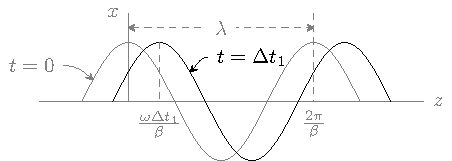
\includegraphics{figWaveMovingRightWithTime}
\caption{وقت $t=0$ اور $t=t_1$ پر خلاء میں موج کا مقام۔}
\label{شکل_موج_وقت_کے_ساتھ_مثبت_چلتی_موج}
\end{figure}

مساوات \حوالہ{مساوات_موج_کوسائن_مثبت_موج} کو وقت \عددیء{t=0} پر شکل \حوالہ{شکل_موج_وقت_کے_ساتھ_مثبت_چلتی_موج} میں ہلکی سیاہی میں دکھایا گیا ہے۔یہاں دھیان رہے کہ شکل میں \عددیء{z} محدد کو افقی دکھایا گیا ہے۔جیسے آپ دیکھ سکتے ہیں \عددیء{t=0} پر موج کی دو آپس میں قریبی چوٹیاں \عددیء{z=0} اور \عددیء{z=\tfrac{2\pi}{\beta}} پر پائی جاتی ہیں۔دو آپس میں قریبی چوٹیوں کے درمیان فاصلے کو \اصطلاح{طول موج}\فرہنگ{طول موج}\فرہنگ{موج!طول}\حاشیہب{wavelength}\فرہنگ{wavelength} پکارا اور \عددیء{\lambda} سے ظاہر کیا جاتا ہے۔یوں اس موج کی طول موج
\begin{align}\label{مساوات_موج_زاویائی_مستقل_اور_طول_موج}
\lambda=\frac{2\pi}{\beta}
\end{align}
ہے۔

مساوات \حوالہ{مساوات_موج_کوسائن_مثبت_موج} ہی کو وقت \عددیء{t=\Delta t_1} پر شکل \حوالہ{شکل_موج_وقت_کے_ساتھ_مثبت_چلتی_موج} میں دوبارہ گاڑھی سیاہی میں بھی دکھایا گیا ہے۔آپ دیکھ سکتے ہیں کہ اس دورانیے میں موج نے دائیں جانب یعنی \عددیء{z} بڑھنے کی طرف حرکت کی ہے۔یوں صاف ظاہر ہے کہ یہ موج وقت کے ساتھ مثبت \عددیء{z} جانب حرکت کر رہی ہے۔ وقت \عددیء{\Delta t_1} میں موج کی چوٹی نے \عددیء{\tfrac{\omega \Delta t_1}{\beta}} فاصلہ طے کیا ہے لہٰذا موج کے رفتار کو
\begin{align}\label{مساوات_موج_رفتار_اور_تعدد}
v=\frac{\Delta z}{\Delta t}=\frac{\omega \Delta t_1}{\beta} \frac{1}{\Delta t_1}=\frac{\omega}{\beta}
\end{align}
لکھا جا سکتا ہے۔

مساوات \حوالہ{مساوات_موج_زاویائی_مستقل_اور_طول_موج} کو \عددیء{\beta=\tfrac{2\pi}{\lambda}} لکھتے ہوئے مساوات \حوالہ{مساوات_موج_رفتار_اور_تعدد} میں پر کرنے سے
\begin{align}
v=f \lambda
\end{align}
حاصل ہوتا ہے جو \عددیء{\lambda} طول موج  اور \عددیء{f} تعدد رکھنے والے موج کی رفتار \عددیء{v} دیتی ہے۔

مساوات \حوالہ{مساوات_موج_کوسائن_مثبت_موج} میں مساوات \حوالہ{مساوات_موج_رفتار_اور_تعدد} استعمال کرتے ہوئے
\begin{align}
E_x=E_0 \cos \left[ \omega \left(t-\frac{z}{v} \right)\right]
\end{align}
حاصل ہوتا ہے۔

موج کی رفتار کو مساوات \حوالہ{مساوات_موج_کوسائن_مثبت_موج} سے دوبارہ حاصل کرتے ہیں۔اس مساوات کے تحت کسی بھی لمحہ \عددیء{t} پر موج کی چوٹی اس مقام پر ہو گی جہاں
\begin{align*}
\omega t -\beta z=0
\end{align*}
ہو۔چونکہ رفتار \عددیء{\tfrac{\dif z}{\dif t}} کو کہتے ہیں لہٰذا اس مساوات کے تفرق
\begin{align*}
\omega \dif t-\beta \dif z=0
\end{align*}
سے رفتار
\begin{align}
v=\frac{\dif z}{\dif t}=\frac{\omega}{\beta}
\end{align}
حاصل ہوتی ہے۔

اگر ہم مساوات \حوالہ{مساوات_موج_منفی_زیڈ_جانب} کو لے کر آگے بڑھتے تو مساوات \حوالہ{مساوات_موج_کوسائن_مثبت_موج} کی جگہ موج کی مساوات
\begin{align}\label{مساوات_موج_کوسائن_منفی_موج}
E_x=E_0 e^{\alpha z} \cos (\omega t +\beta z)
\end{align}
حاصل ہوتی۔یہ موج \عددیء{z} محدد پر منفی جانب حرکت کر رہی ہے اور ایسا کرتے ہوئے اس کی چوٹی آہستہ آہستہ کم ہو رہی ہے۔
